%%%%%%%%%%%%%%%%%%%%%%%%%%%%%%%%%%%%%%%%%%%%%%%%%%%%%%%%%%%%%%%%%%%%%%%%%%%
%%%             DESCRICOES TEORICAS E FERRAMENTAS BASICAS               %%%
%%%%%%%%%%%%%%%%%%%%%%%%%%%%%%%%%%%%%%%%%%%%%%%%%%%%%%%%%%%%%%%%%%%%%%%%%%%

\setlength{\parskip}{0.3cm}

\chapter{Capítulo 2~-~Fundamentação Teórica}~\label{ch:fundamentacao}

\section{Biologia Molecular}
A Biologia Molecular é um ramo da biologia que lida e investigas os processos e mecanismos moleculares relacionados à estrutura, função e interações das biomoléculas presentes nos organismos vivos. Consiste em principalmente em estudar as interações entre os vários sistemas da célula, partindo da relação entre o \gls{dna}, \gls{rna} e a síntese de proteínas, e o modo como essas interações são reguladas.

É importante entender a estrutura do \gls{dna} vista na Figura~\ref{fig:estruturaDNA}, está é uma molécula em forma de dupla hélice que carrega a informação genética em organismos vivos. Ela é composta por duas cadeias polinucleotídicas complementares enroladas em torno de um eixo central. Cada cadeia é composta por uma sequência de nucleotídeos, que consistem em uma pentose (a desoxirribose), um grupo fosfato e uma base nitrogenada (adenina, timina, citosina ou guanina). A estrutura do \gls{dna} é mantida por pontes de hidrogênio entre as bases complementares, com a adenina pareando sempre com a timina e a citosina pareando sempre com a guanina.

%%figura
\begin{figure}[htb]
  \centering
  \caption{Estrutura do DNA.}
  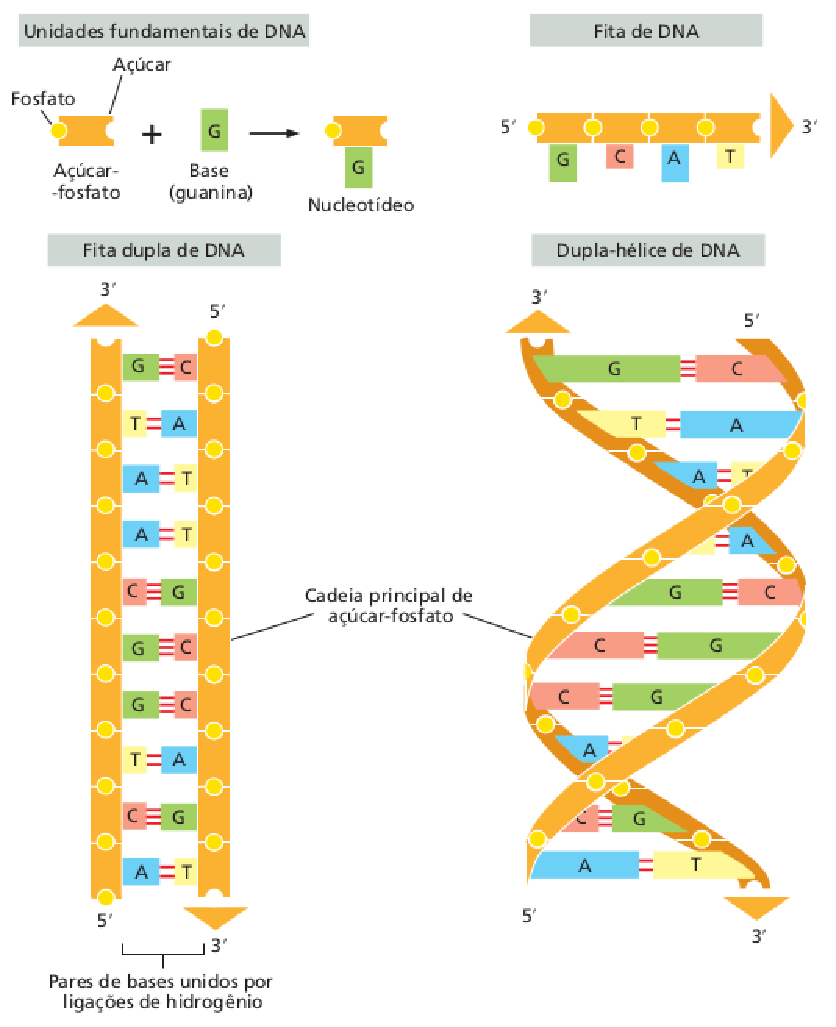
\includegraphics[scale=0.6]{figuras/estruturaDNA_02.pdf}
  \fonte{Retirada de \citeauthor{alberts_biologia_2017}}~\label{fig:estruturaDNA}
\end{figure}

As informações contidas no \gls{dna} é copiada em uma molécula de \gls{rna}, esse processo é conhecido como transcrição. A transcrição ocorre no núcleo das células e envolve a separação das duas fitas do \gls{dna} e o pareamento de nucleotídeos complementares para sintetizar uma molécula de \gls{mrna}. O \gls{mrna} é uma cópia do DNA que carrega a sequência de bases nitrogenadas correspondente a um gene específico.
Após isso, ocorre o processo de tradução onde a sequência de bases nitrogenadas do \gls{mrna} é utilizada para sintetizar proteínas. A tradução ocorre nos ribossomos, presentes no citoplasma celular. Durante a tradução, o \gls{mrna} é lido em grupos de três bases, chamados de códons. Cada códon especifica um aminoácido distinto. Os aminoácidos são transportados para o ribossomo por moléculas de \gls{trna}, que possuem um anticódon complementar ao códon do \gls{mrna}. À medida que o ribossomo percorre o \gls{mrna}, os aminoácidos são ligados em uma sequência específica, formando uma cadeia polipeptídica que será dobrada e modificada para se tornar uma proteína funcional~\cite{alberts_biologia_2017}.

\section{Virus}

Os vírus são agentes infecciosos compostos por uma cápsula proteica (capsídeo) que envolve seu material genético, que pode ser \gls{dna} ou \gls{rna}.
A estrutura viral varia entre diferentes tipos de vírus, mas de modo geral, eles consistem em uma cápsula proteica chamada capsídeo, que envolve o material genético viral. O capsídeo pode apresentar diferentes formas, como hélices, icosaedros ou formas complexas. Além do capsídeo, alguns vírus possuem uma camada lipídica chamada envelope viral, que é derivada da membrana da célula hospedeira e contém glicoproteínas virais que são importantes para a entrada do vírus nas células hospedeiras~\cite{david_virology_2022}.
O ciclo e vida viral é conjunto de etapas que um vírus passa para se reproduzir e infectar novas células. Esse ciclo pode variar entre diferentes tipos de vírus, mas geralmente envolve as seguintes etapas:

\begin{enumerate}
  \item Adsorção: o vírus se liga especificamente a receptores na superfície da célula hospedeira.
  \item Penetração: o vírus entra na célula hospedeira, liberando seu material genético.
  \item Replicação e síntese de proteínas virais: o material genético viral é replicado e transcritas em moléculas de \gls{mrna}, que são utilizadas para a síntese de proteínas virais
  \item Montagem: as proteínas virais se unem para formar novas partículas virais
  \item Liberação: as novas partículas virais são liberadas da célula hospedeira, podendo ocorrer por lise celular ou por brotamento
\end{enumerate}

\subsection{SARS-CoV-2}

O SARS-CoV-2 é um vírus da família Coronaviridae, que causa a doença chamada \gls{covid19}. Ele foi identificado pela primeira vez em dezembro de 2019 na cidade de Wuhan, na província de Hubei, na China, e desde então se espalhou para todo o mundo, resultando em uma pandemia global~\cite{zhu_novel_2020,wu_coronavirus_2020}.

O SARS-CoV-2 possui uma estrutura viral apresentada na Figura~\ref{fig:estruturaCoronavirus}, característica dos coronavírus. Ele é composto por uma partícula viral esférica, com um envelope lipídico que envolve seu material genético. A estrutura do vírus inclui proteínas de espículas na sua superfície, conhecidas como proteína spike (S), que são responsáveis pela ligação do vírus às células hospedeiras. Além disso, o SARS-CoV-2 possui proteínas de membrana (M), envelope (E) e nucleocapsídeo (N), que desempenham papéis importantes na estrutura e na replicação viral.

\begin{figure}[htb]
  \centering
  \caption{Estrutura do coronavírus.}
  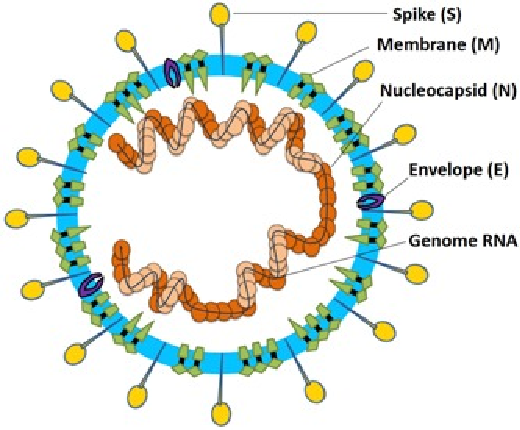
\includegraphics[scale=0.8]{figuras/estruturaSarsCov2.pdf}
  \fonte{Retirada de \citeauthor{li_coronavirus_2020}}~\label{fig:estruturaCoronavirus}
\end{figure}

\section{Filogenia}

A filogenia é uma disciplina da biologia que estuda as relações evolutivas entre organismos, buscando reconstruir a história evolutiva e a ancestralidade comum. A filogenética molecular é uma abordagem utilizada para inferir a filogenia com base em informações moleculares, como sequências de \gls{dna}, \gls{rna} e proteínas\cite{felsenstein_inferring_2004}.

A construção de árvores filogenéticas é um aspecto fundamental da filogenética molecular. Existem vários métodos utilizados para construir árvores filogenéticas, que podem ser classificados em dois grupos principais: métodos baseados em distância e métodos baseados em caracteres.
Os métodos baseados em distância medem a similaridade ou a dissimilaridade entre sequências moleculares e constroem árvores filogenéticas com base nessas medidas. Alguns exemplos de métodos baseados em distância incluem o método de Neighbor Joining (NJ) e o método de Mínima Evolução (ME).
Por outro lado, os métodos baseados em caracteres analisam as mudanças nos caracteres moleculares ao longo do tempo para inferir as relações filogenéticas. Exemplos de métodos baseados em caracteres são o método de Máxima Parcimônia (MP) e o método de Inferência Bayesiana\cite{swofford_phylogenetic_1996}.

% \section{Bioinformática}

% Alinhamento de Sequências, Análise de Genomas Virais, Análise de Expressão Gênica, Ferramentas de Bioinformática

% Para iniciar, vamos testar novamente o uso de siglas: \gls{AA}. Observe que mesmo ao iniciar outro capítulo, a sigla não precisa ser definida novamente por extenso, pois já foi definida no capítulo anterior, além de estar definida na lista de siglas e abreviaturas.

% A partir do capítulo~\ref{ch:fundamentacao} começa-se a apresentar a fundamentação teórica. Atenção ! Fundamentação teórica não é o mesmo que trabalhos relacionados ou estado da arte. Fundamentação teórica são conceitos teóricos - alguns mesmo antigos ou clássicos - que precisam ser compreendidos para entender a solução apresentada para o problema investigado.

% Não há um modelo de divisão de capítulos. Alguns autores criam um único capítulo chamado `Fundamentação Teórica' e nele colocam todos os conteúdos divididos em seções, subseções, etc. Outros preferem criar capítulos diferentes para temas diferentes da fundamentação teórica. Enfim, não há uma regra rígida para isto. Deve ser definido em consenso com o orientador. O importante é ter bom senso para não criar vários capítulos minúsculos com 1 página ou menos. Se o que tem para falar de um tema é tão pouco, talvez valha à pena ter um único capítulo de fundamentação teórica com várias seções falando dos diversos temas que compõem sua fundamentação. Mas se cada tema tem muito a ser falado, pode ficar melhor dividi-los em capítulos diferentes.

% Quanto a Trabalhos Relacionados ou Estado da Arte eles são as publicações recentes de pessoas que tentaram resolver o mesmo problema ou um problema similar. São o resultado da revisão sistemática de literatura feita no início do processo de TCC. Alguns autores optam por fazer a análise destes trabalhos dentro do capítulo de introdução. Outros optam por criar um capítulo denominado "Estado da Arte" ou "Revisão de Literatura" ou "Trabalhos Relacionados" e fazer esta análise lá. A decisão mais uma vez fica a critério de cada autor e deve ser tomada em consenso com o orientador. Se os Trabalhos Relacionados estiverem na introdução, certamente irá gerar uma introdução mais longa. Mas não há problema ou impedimento quanto a isto.

% Uma vantagem de colocar na introdução é que logo no início da monografia já ficam claras as lacunas do estado da arte que seu trabalho buscará preencher. Quando feito num capítulo à parte isto só aparece depois, mas gera o benefício de não deixar a introdução tão extensa e por vezes cansativa para o leitor. Então é uma questão de decisão do autor e do orientador.

% Quando colocado num capítulo à parte costuma vir antes dos capítulos de fundamentação teórica.